\chapter{Implementation}
\label{ch:whatYouDid}

\com{
\todo[inline]{Choose your own chapter title to describe this}

\todo[inline]{What have you done? How did you do it? What design decisions did you make? How did what you did help you to meet your goals?}



Describe the engineering-related contents (preferably with models) and the research methodology and methods that are used in the degree project.

Give a theoretical description of the scientific or engineering methodology are you going to use and why have you chosen this method. What other methods did you consider and why did you reject them.

In this chapter, you describe what engineering-related and scientific skills you are going to apply, such as modeling, analyzing, developing, and evaluating engineering-related and scientific content. The choice of these methods should be appropriate for the problem . Additionally, you should be consciousness of aspects relating to society and ethics (if applicable). The choices should also reflect your goals and what you (or someone else) should be able to do as a result of your solution - which could not be done well before you started.

The purpose of this chapter is to provide an overview of the research method
used in this thesis. Section~\ref{sec:researchProcess} describes the research
process. Section~\ref{sec:researchParadigm} details the research
paradigm. Section~\ref{sec:dataCollection} focuses on the data collection
techniques used for this research. Section~\ref{sec:experimentalDesign}
describes the experimental design. Section~\ref{sec:assessingReliability}
explains the techniques used to evaluate the reliability and validity of the
data collected. Section~\ref{sec:plannedDataAnalysis} describes the method
used for the data analysis. Finally, Section~\ref{sec:evaluationFramework}
describes the framework selected to evaluate xxx.

}
DRAFT

\noindent

RISE AB, in collaboration with Husqvarna AB, is interested in the research and development of a refined approach to improve the performance of the \gls{ALM}, thus allowing for the development of more features.
The system will be built upon the \Gls{HRP}~\cite{HRP}, a \Gls{ROS} enabled Husqvarna Automower 450X with additional sensors assembled upon it, as shown in Figure \ref{fig:HardwareSetup}.
It has been improved by a former thesis student~\cite{HRPTianze} and it is now equipped with additional two \Glspl{IMU}, two \Gls{GNSS} signal receivers, and a \Gls{RGBD} camera.

\begin{figure}[!ht]
	\begin{center}
		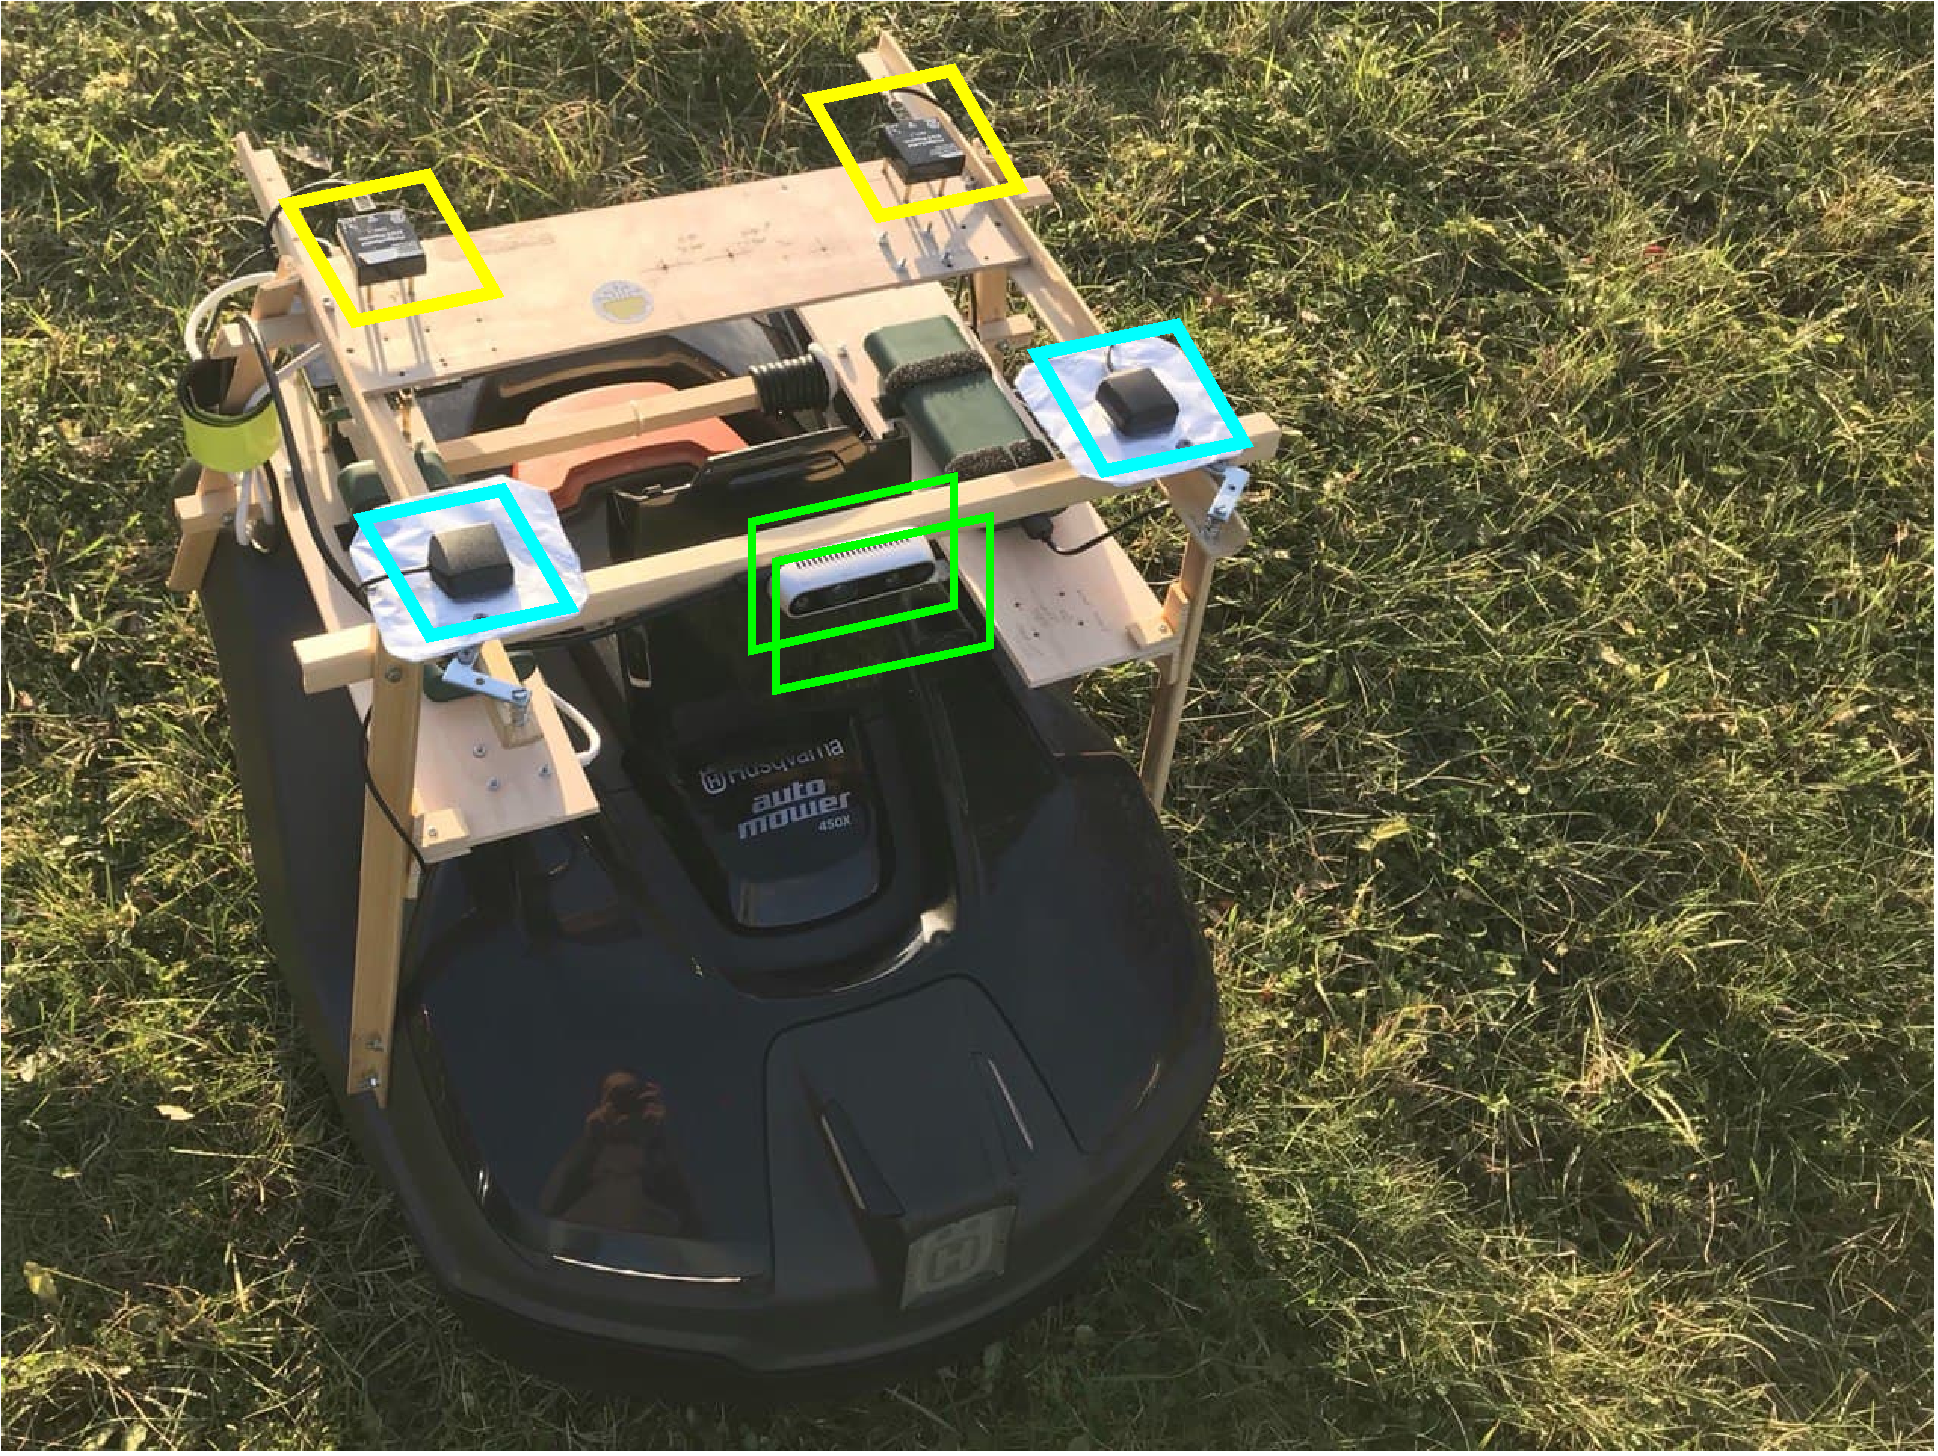
\includegraphics[width=1.0\textwidth]{Images/1-Introduction/projectTheme.pdf}
		\caption{
			\gls{ALM} Model with focus on additional sensors:\\
		    \glspl{IMU} [yellow], \gls{GNSS} receivers [cyan], and Camera [green]
	\centering }
		\label{fig:HardwareSetup}
	\end{center}
\end{figure}


The platform adopted, \gls{HRP}, has been improved starting from its configuration and sensors' drivers.


At first, an analysis of available platform is performed to gain a more comprehensive understanding of the current \gls{HRP} implementation.
The documentation of the \gls{HRP}~\cite{HRP} and by the previous student~\cite{HRPTianze} are going to be carefully comprehended before focusing on the study of the related state-of-the-art.


\section{Hardware Configuration}
\label{sec:system}

\noindent
\gls{HRP} that holds the sensors and the raspberry pi, also proving the measurements of the wheel encoders and of the embedded GPS receiver.
Computer to guide the \gls{ALM} and make him move according to the desired path, also at the end the \gls{ALM} was free to run its random path and use the algorithm implemented to stay inside the boundaries.

\com{
\begin{figure}[!ht]
  \begin{center}
    \includegraphics[width=0.5\textwidth]{Images/4-Done/}
  \end{center}
  \caption{Hardware}
  \label{fig:hardware}
\end{figure}
}


\com{
	\subsection{Devices}
	\label{ssec:dev}
	\noindent
	Raspberry Pi 4 to guide the \gls{ALM}, to gather information about the topics of ROS, and to communicate them to the personal computer used to gather them.
}

\subsection{Raspberry Pi 4}
\noindent
On this device, most of the embedded devices will be attached.
The \gls{HRP}, the \glspl{IMU}, and the camera.

\begin{figure}[!ht]
	\begin{center}
		\begin{subfigure}[b]{.5\textwidth}
			\begin{center}
				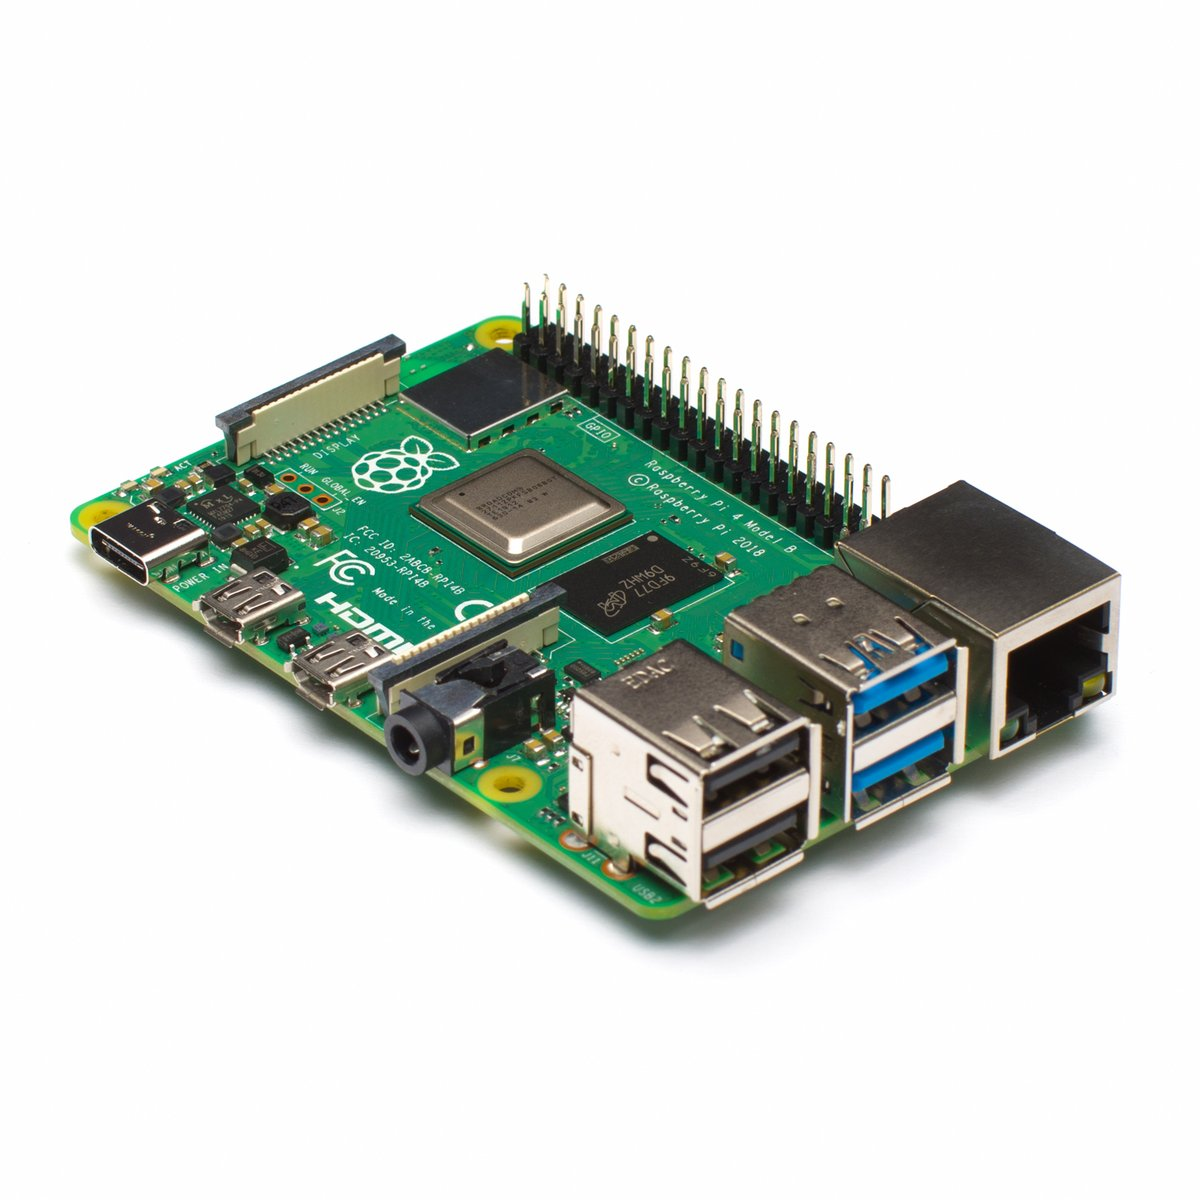
\includegraphics[width=0.85\textwidth]{Images/4-Methods/RPi4.jpg}
			\end{center}
			\caption{Raspberry Pi 4 Model B}
			\label{fig:rpi4Im}
		\end{subfigure}
		\begin{subfigure}[b]{.45\textwidth}
			\begin{center}
				\begin{tikzpicture}[font=\small,thick]
					\node[draw, text centered, fill=white!30,
					align=center,
					minimum width=3cm,
					minimum height=1cm,
					] (block0) { Raspberry Pi 4};
					
					\node[draw,text centered,fill=white!30,rounded corners,
					below=0.5cm of block0, align=center,
					minimum width=2.5cm,
					minimum height=1cm,
					] (block1) { \gls{HRP} Automower };
					
					\node[above=of block0] (block) { };
					
					\node[draw,text centered,fill=yellow!30,rounded corners,
					left=0.1cm of block,
					align=center,
					minimum width=2.5cm,
					minimum height=1cm,
					] (block2) { Phidget \glspl{IMU}};
					
					\node[draw,text centered,fill=green!30,rounded corners,
					right=0.1cm of block,
					align=center,
					minimum width=2.5cm,
					minimum height=1cm,
					] (block3) { Camera};
					
					\node[below=of block1] (blockk) { };
					
					\node[draw,text centered,fill=white!30,rounded corners,
					left=0.1cm of blockk,
					align=center,
					minimum width=2.5cm,
					minimum height=1cm,
					] (block4) { Wheel Encoder};
					
					\node[draw,text centered,fill=white!30,rounded corners,
					right=0.1cm of blockk,
					align=center,
					minimum width=2.5cm,
					minimum height=1cm,
					] (block5) { Automower \gls{GNSS}};
					
					% Arrows
					\draw[latex-] (block0) edge (block1);
					\draw[latex-] (block0) edge (block2);
					\draw[latex-] (block0) edge (block3);
					\draw[latex-] (block1) edge (block4);
					\draw[latex-] (block1) edge (block5);
				\end{tikzpicture}
				\caption[Caption]{Raspberry Pi 4 configuration \centering}
			\end{center}
			\label{fig:RPi4Conf}
		\end{subfigure}
		\caption{Raspberry Pi 4}
		\label{fig:RPi4}
	\end{center}
\end{figure}


\subsection{Raspberry Pi 3}
\noindent
On this device, running Ubuntu 20, the Phidgets GPS sensors will be attached.


\begin{figure}[!ht]
	\begin{subfigure}[b]{.5\textwidth}
		\begin{center}
			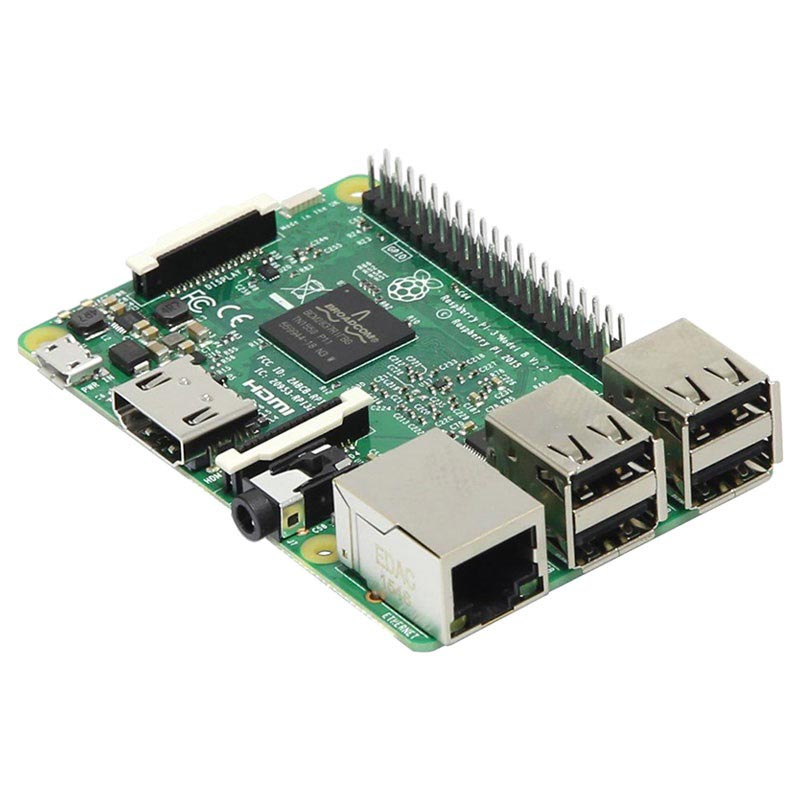
\includegraphics[width=0.5\textwidth]{Images/4-Methods/RPi3.jpg}
		\end{center}
		\caption{Raspberry Pi 3 Model B}
		\label{fig:rpi3Im}
	\end{subfigure}%
	\begin{subfigure}[b]{.45\textwidth}
		\begin{center}
			\begin{tikzpicture}[font=\small,thick]
				\node[draw, text centered, fill=white!30,
				align=center,
				minimum width=3cm,
				minimum height=1cm,
				] (block0) { Raspberry Pi 3};
				
				\node[draw,text centered,fill=cyan!30,rounded corners,
				above=0.5cm of block0, align=center,
				minimum width=2.5cm,
				minimum height=1cm,
				] (block1) { Phidget \glspl{GPS} };
				% Arrows
				\draw[latex-] (block0) edge (block1);
			\end{tikzpicture}
			\caption[Caption]{Raspberry Pi 3 configuration \centering}
		\end{center}
		\label{fig:RPi3Conf}
	\end{subfigure}
	\caption{Raspberry Pi 3}
	\label{fig:RPi3}
\end{figure}

\com{
\subsection{Sensors}
\label{ssec:sens}
\noindent
The following set of sensors are available for fusion using the \gls{AEKF} defined in \ref{ch:methods}.
}

\subsection{Wheel Encoder}
\noindent
It is included in the motor of the wheel of the \gls{ALM}, inside the Motor Kit shown in \ref{fig:wheelenc}.
Measure the wheel displacement and provide \gls{WO}, as explained in \ref{ch:methods}.


The performances have been examined and are available below.

\begin{figure}[!ht]
	\begin{center}
		\begin{subfigure}[b]{.5\textwidth}
			\centering
			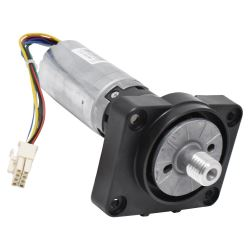
\includegraphics[width=0.75\textwidth]{Images/4-Methods/MotorEnc.jpeg}
			\caption{Motor Kit Automower 450X }
			\label{fig:wheelenc}
		\end{subfigure}%
		\begin{subfigure}[b]{.45\textwidth}
				\begin{center}
					\label{tab:evalWheels}
					\begin{tabular}{|c||S|}
						\hline
						\centering{\textbf{Aspect}} &  \multicolumn{1}{c|}{\textbf{Value}} \\
						\hline
						\hline
						\centering{Frequency} &  \SI{200}{Hz} \\
						\hline
						\centering{$\boldsymbol \eta_v$} &  \SI{0.02}{\meter/\second} \\
						\hline
						\centering{$\boldsymbol \eta_{\omega}$} & \SI{0.02}{\radian/\second} \\
						\hline
					\end{tabular}
					\caption{Sensor's performance}
				\end{center}
		\end{subfigure}
		\caption{Wheel Encoder }
		\label{fig:wheel}
	\end{center}
\end{figure}

They are mounted in the wheel axis on both wheels.

\subsection{Global Navigation Satellite System}

\noindent Measure the satellite positions to estimate its absolute position global values in the global coordinate frame.

Different \glspl{GNSS} are available.
A \gls{GPS} receiver is embedded in the \gls{HRP}, shown in \ref{fig:autogps}.
Moreover, two additional \gls{GPS} receivers has been added, shown in \ref{fig:phigps}.

\begin{figure}[!ht]
\begin{center}
	\begin{subfigure}[b]{.5\textwidth}
		\centering
		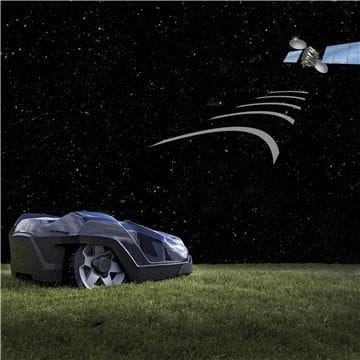
\includegraphics[width=0.75\textwidth]{Images/4-Methods/AutomowerGPS.jpeg}
		\caption{Automower 450X GPS}
		\label{fig:autogps}
	\end{subfigure}%
	\begin{subfigure}[b]{.45\textwidth}
		\begin{center}
			\label{tab:evalAutoGPS}
			\begin{tabular}{|c||S|}
				\hline
				\centering{\textbf{Aspect}} &  \multicolumn{1}{c|}{\textbf{Value}} \\
				\hline
				\hline
				\centering{Frequency} &  \SI{1}{Hz} \\
				\hline
				\centering{$\boldsymbol \eta_x$} &  \SI{0.02}{\meter/\second} \\
				\hline
				\centering{$\boldsymbol  \eta_y$} &  \SI{0.02}{\meter/\second} \\
				\hline
				\centering{$\boldsymbol \eta_{\theta}$} & \SI{0.02}{\radian/\second} \\
				\hline
			\end{tabular}
			\caption{Sensor's performance}
		\end{center}
	\end{subfigure}
	\caption{\glspl{GNSS} receivers adopted}
	\label{fig:gpssensorauto}
\end{center}
\end{figure}

The performances of PhidgetGPS ID: 1040\_0B have been examined and are available below.

\begin{figure}[!ht]
	\begin{center}
		\begin{subfigure}[b]{.5\textwidth}
			\centering
			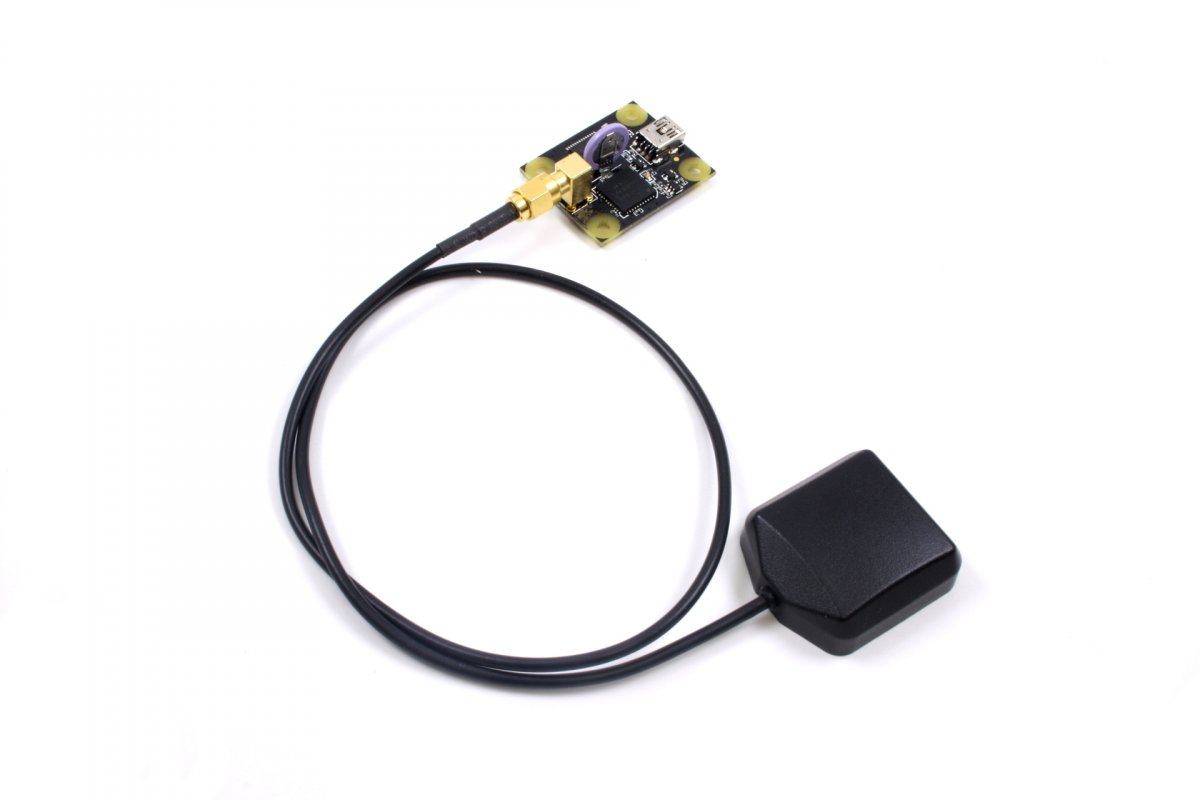
\includegraphics[width=1\textwidth]{Images/4-Methods/1040_0B_Alt2.jpg}
			\caption{Phidget GPS}
			\label{fig:phigps}
		\end{subfigure}
		\begin{subfigure}[b]{.45\textwidth}
			\begin{center}
				\label{tab:evalPhiGPS}
				\begin{tabular}{|c||S|}
					\hline
					\centering{\textbf{Aspect}} &  \multicolumn{1}{c|}{\textbf{Value}} \\
					\hline
					\hline
					\centering{Frequency} &  \SI{5}{Hz} \\
					\hline
					\centering{$\boldsymbol \eta_x$} &  \SI{0.02}{\meter/\second} \\
					\hline
					\centering{$\boldsymbol  \eta_y$} &  \SI{0.02}{\meter/\second} \\
					\hline
					\centering{$\boldsymbol \eta_{\theta}$} & \SI{0.02}{\radian/\second} \\
					\hline
				\end{tabular}
				\caption{Sensor's performance}
			\end{center}
		\end{subfigure}%
		\caption{\glspl{GNSS} receivers}
		\label{fig:gpssensorphi}
	\end{center}
\end{figure}



It is mounted in front, at coordinate x,y,z with orientation theta with respect to the robot coordinate frame.

\subsection{Inertial Measurement Unit}

\noindent Measure the angular velocity, acceleration, and magnetic fields in the three orthogonal axis.

This PhidgetSpatial Precision 3/3/3 High Resolution - ID: 1044\_1B, shown in \ref{fig:spatial}, has a 3-axis accelerometer, gyroscope and compass with high resolution readings at low magnitudes.

The performances have been examined and are available below.

\begin{figure}[!ht]
	\begin{center}
		\begin{subfigure}[b]{.5\textwidth}
			\begin{center}
				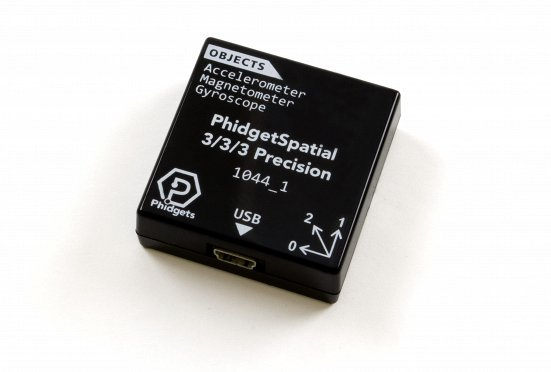
\includegraphics[width=1\textwidth]{Images/4-Methods/1044_1B.jpg}
			\end{center}
			\caption{PhidgetSpatial}
			\label{fig:spatial}
		\end{subfigure}
		\begin{subfigure}[b]{.45\textwidth}
			\begin{center}
				\label{tab:evalPhiIMU}
				\begin{tabular}{|c||S|}
					\hline
					\centering{\textbf{Aspect}} &  \multicolumn{1}{c|}{\textbf{Value}} \\
					\hline
					\hline
					\centering{Frequency} &  \SI{250}{Hz} \\
					\hline
					\centering{$\boldsymbol \eta_{\omega}$} & \SI{0.02}{\radian/\second} \\
					\hline
					\centering{$\boldsymbol \eta_{a}$} & \SI{0.02}{\meter/\second \squared} \\
					\hline
				\end{tabular}
				\caption{Sensor's performance}
			\end{center}
		\end{subfigure}%
		\caption{\glspl{IMU}}
		\label{fig:imusensorphi}
	\end{center}
\end{figure}

It is mounted in front, at coordinate x,y,z with orientation theta with respect to the robot coordinate frame.

\subsection{RGB-D Camera}

\noindent Measure the displacement of the camera \gls{F2F} and provide \gls{VO}.
The device that is used is the Intel® RealSense™ depth camera D435, shown in Figure \ref{fig:d435}.
It provides \gls{RGBD} images, i.e. both \gls{RGB} and depth information.

"The Intel® RealSense™ depth camera D435 is a stereo solution, offering quality depth for a variety of applications. It's wide field of view is perfect for applications such as robotics or augmented and virtual reality, where seeing as much of the scene as possible is vitally important."

\begin{figure}[!ht]
	\begin{center}
		\begin{subfigure}[b]{.5\textwidth}
			\begin{center}
				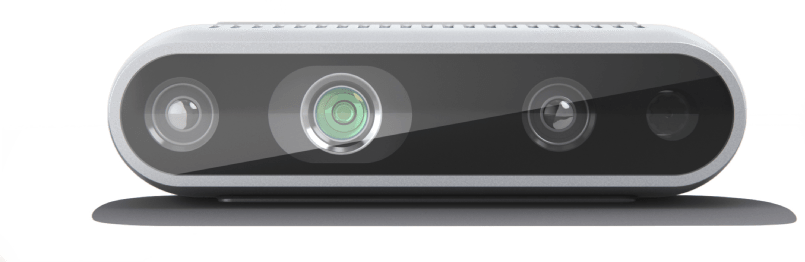
\includegraphics[width=0.85\textwidth]{Images/4-Methods/d435i-1.png}
			\end{center}
			\caption{\gls{RGBD} Camera}
			\label{fig:d435}
		\end{subfigure}
		\begin{subfigure}[b]{.45\textwidth}
			\begin{center}
				\label{tab:evalCamera}
				\begin{tabular}{|c||S|}
					\hline
					\centering{\textbf{Aspect}} &  \multicolumn{1}{c|}{\textbf{Value}} \\
					\hline
					\hline
					\centering{Frequency} &  \SI{5}{Hz} \\
					\hline
					\centering{$\boldsymbol \eta_{v}$} & \SI{0.02}{\meter/\second} \\
					\hline
					\centering{$\boldsymbol \eta_{\omega}$} & \SI{0.02}{\radian/\second} \\
					\hline
				\end{tabular}
				\caption{Sensor's performance}
			\end{center}
		\end{subfigure}%
		\caption{Camera}
		\label{fig:camera_sensor}
	\end{center}
\end{figure}

It is mounted in front, at coordinate x,y,z with orientation theta with respect to the robot coordinate frame.

Using the \gls{RTABMAP} package\footnote{\url{http://introlab.github.io/rtabmap/}}\cite{6094602} \cite{labbe_rtab-map_2019}, more specifically the \gls{ROS} version 0.20.9 for \gls{ROS} Noetic.

\section{Software Configuration}
\noindent
C++ and Python development to work with the ROS framework, explained in details in Appendix \ref{ch:ros}.

Network establishment to communicate wirelessly between Raspberry Pi and computer.

Communication through hotspot



\subsection{Controller}
\label{sec:driver_safe}
\noindent The \gls{ALM} behaviour is defined by the launching file \texttt{automower\_hrp.launch}.
It defines and launch the controller of the \gls{HRP}.



\subsection{Velocity Control}
\label{sec:control}
\noindent
The script \texttt{hrp\_teleop.lauch} as provided by the \gls{HRP} platform is used to drive the \gls{ALM} during the experiments.
It controls the vehicle by setting its desired velocities: $\mathbf{v}v$ and $\boldsymbol \omega$.
In this way it is possible to command the \gls{ALM} to follow a trajectory.


\subsection{Launching the sensors}
\noindent The measurements are obtained from the heterogeneous sensors using the following methods.


The \glspl{IMU} sensors are started using the file \texttt{imus\_basic.launch}.
In this file, the node defined by the \texttt{phidget\_spatial} drivers is used, each sensor will belong to its group, and its coordiante frame is defined by the installation coordinates.

The additional Phidget \gls{GPS} sensors are launched by the file \texttt{imus\_basic.launch}.
In the file, the node calls for a personalised driver that has been implemented to gather the \gls{NMEA} data directly provided by the Phidgets \gls{API}.
The information provided by this \gls{NMEA} data structure

The additional Phidget \gls{GPS} sensors are launched by the file \texttt{imus\_basic.launch}.
In the file, the node calls for a personalised driver that has been implemented to gather the \gls{NMEA} data directly through the Phidgets \gls{API}.
The information provided by this \gls{NMEA} data structure covers both the localisation estimate and its related accuracy, in form of \gls{HDOP}.

The camera added is exploited running the file \texttt{rs\_camera.launch}.
It is a customised launch file that has been improved starting from the camera own driver.
As it does not provide the measurements directly, the \gls{VO} package \gls{RTABMAP} is run via a customised \texttt{rtabmap.launch} file, obtained initially from the \gls{RTABMAP} package and then tuned for the scope of this thesis.



\subsection{Launching the localisation feature}
\noindent The localisation improvements are performed by the script in \texttt{AEKF.py}.
It performs the \gls{AEKF} elaborated in \ref{sec:locConf}.

To perform in an asynchronous way, a binary lock is adopted to account when a measurement update is performed at the same time of a measurement receive.


\subsection{Launching the mapping update}
\noindent The mapping feature is provided by the implementation available in \texttt{Mapping.py}.

The initial phase is of setting the boundaries.

Then a specific message changes the

The collision events are then exploited to update the knowledge of the surroundings.





\cleardoublepage
%\clearpage
